\section*{\textbf{METHODS AND RESULTS}}

For our experiments, we have chosen two classical algorithms: Canny edge detector and grayscale morphology, namely, dilation with the disk structuring element. Both of them are often used in industrial recognition systems (e.g. \cite{panfilova2020using}, \cite{panfilova2021fast}, \cite{erlygin2021improvement}). There is a baseline on an approximation of Canny operator \citep{Fernandez11}, but there was a feedforward neural network used, while research for convolutional neural networks was not conducted. And, as far as we are concerned, there are no published studies for approximation of morphological dilatation. Moreover, there is no computationally efficient implementation of dilation with the disk structuring element compared, at least, to the rectangular structuring element, for which fast window size-independent algorithm (vHGW) is available~\citep{limonova2020fast}.

Furthermore, we want to investigate two different approaches to approximating filters: regression and classification. As long as Canny detects edges on the image, it might be considered as a classification of each pixel whether it is a part of an edge or not. On the other hand, morphological filters do not \glqq classify\grqq each pixel; instead, they process an input image to another one, which might be considered as a regression. 

\subsection*{\textbf{Approximation with fixed parameters}}

% At first, we wanted to test the ability of the neural networks to approximate a particular filter with specified parameters. For Canny edge detector, we specified these parameters as $\sigma=1$, low threshold = 0.1, high threshold = 0.2. For morphological dilation, we approximated filter with two sizes of filter's radius: $R_1 = 5$ as a baseline and $R_2 = 20$ to be sure that the receptive field of the network is large enough to approximate dilation with a big radius. 

At first, we wanted to test the ability of the neural networks to approximate a particular filter with specified parameters. There are three key parameters of Canny edge detector \citep{CannyPaper}: standard deviation for Gaussian kernel $\sigma$, lower bound for hysteresis thresholding (low threshold), and upper bound for hysteresis thresholding (high threshold). We specified these parameters as $\sigma=1$, low threshold = 0.1, high threshold = 0.2. For morphological dilation, we approximated the filter with two sizes of the radius: $R_1 = 5$ as a baseline and $R_2 = 20$ to be sure that the receptive field of the network is large enough to approximate dilation with a big radius. 
%\citep{CannyPaper}

We tried three architectures: ConvNet, which is a stack of convolutional layers with ReLU as activation function, ResNet, and UNet. These architectures might be considered as the gold standard of convolutional networks because they are well-known and often used in many cases of image processing and computer vision \citep{CNNSurvey}. We considered only the most typical neural network architectures without optimizing them for a particular filter. The reason is that our study aims to investigate the universality of standard neural network models for solving classical image processing problems for which there already exists a well-working analytical algorithm.  

%Мы рассматривали только наиболее типовые архитектуры нейронных сетей,не  пытаясь  оптимизировать  ее  под  конкретный фильтр,  потому  что  наша  цель  заключается  висследовании универсальности применения стандартныхнейросетевых моделей для решения классическихзадач,  для  которых  уже  существует  хорошо работающее аналитическое решение

As we mentioned earlier, the problem of Canny edge detector approximation can be formulated in terms of a pixel-by-pixel classification, thus we used the binary cross-entropy loss function. The metrics are Matthew's correlation coefficient, or MCC, \citep{TubeCountour}, and Intersection over Union, or IoU,  \citep{EdgeDetectionIOU}. For morphological dilation approximation, we used the mean squared error loss function and mean absolute error as a metric. Also, we compared different models using the loss function value on the test dataset. 

For each filter, all three networks were trained with the same hyperparameters. Particularly, we used Adam optimizer with learning rate 0.001 and parameters $\beta_1 = 0.9, \beta_2 = 0.999$; cosine annealing scheduler with warm restarts with a period of 8 epochs; 50 epochs for training. As the dataset, we used Linnaeus5 with images of size 128x128 pixels split into training, validation, and test sets with 6000, 1000, and 1000 images, respectively. 

All three models showed comparable results for morphology approximation, but for Canny detector approximation, the best quality was achieved with ResNet (table \ref{table:MetricsCanny}), that is why in the following experiments we used only this architecture. Our implementation of ResNet reproduces the classic implementation and differs only in the number of layers and the number of filters in convolutional layers. It consists of 7 residual blocks, each of them containing 2 convolutional layers with 12 filters. A visualization of the ResNet work is shown in the fig. \ref{figure:Canny} and fig. \ref{figure:Morphology} for Canny edge detector and grayscale morphology with the disk structuring element, respectively.

\begin{table}[h]
\scalebox{0.92}{
\begin{tabular}{|c|c|ccc|}
\hline
\multirow{3}{*}{Model} & \multirow{3}{*}{\begin{tabular}[c]{@{}c@{}}Num. \\ of \\ parameters\end{tabular}} & \multicolumn{3}{c|}{Metrics}                                                                                  \\ \cline{3-5} 
                       &                                                                                   & \multicolumn{1}{c|}{\multirow{2}{*}{MCC}} & \multicolumn{1}{c|}{\multirow{2}{*}{IoU}} & \multirow{2}{*}{Test BCE} \\
                       &                                                                                   & \multicolumn{1}{c|}{}                     & \multicolumn{1}{c|}{}                     &                       \\ \hline
ConvNet                & 25.8k                                                                             & \multicolumn{1}{c|}{0.9185}               & \multicolumn{1}{c|}{0.9230}               & 0.0462                \\ \hline
ResNet                 & 29.1k                                                                             & \multicolumn{1}{c|}{\textbf{0.9286}}      & \multicolumn{1}{c|}{\textbf{0.9322}}      & \textbf{0.0425}       \\ \hline
UNet                   & 28.7k                                                                             & \multicolumn{1}{c|}{0.8291}               & \multicolumn{1}{c|}{0.8481}               & 0.1020                \\ \hline
\end{tabular}}
\caption{Metrics for Canny edge detector approximation}
\label{table:MetricsCanny}
\end{table}

\begin{figure*}[h]
\centering
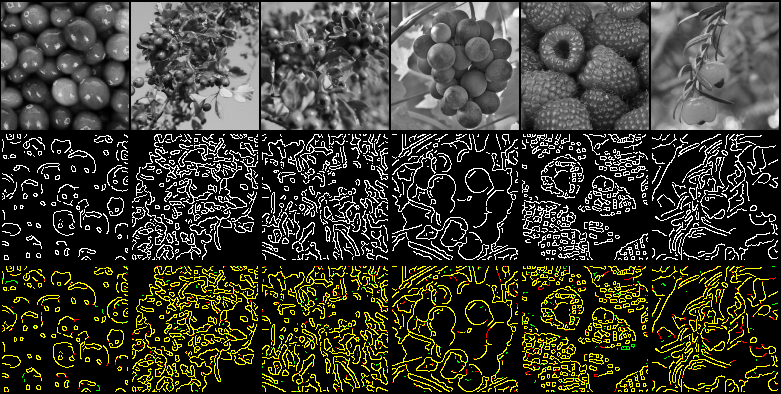
\includegraphics[width=0.85\linewidth]{fig/canny fixed2.png}
\caption{Approximation of Canny edge detector with fixed parameters (1-st row: original images, 2-st row: Canny edge detector, 3-st row: pixel difference with the neural network output, where black, yellow, green, and red colours stand for true negative, true positive, false positive, and false negative pixels, respectively).}
\label{figure:Canny}
\end{figure*}


\begin{figure*}[h]
\centering
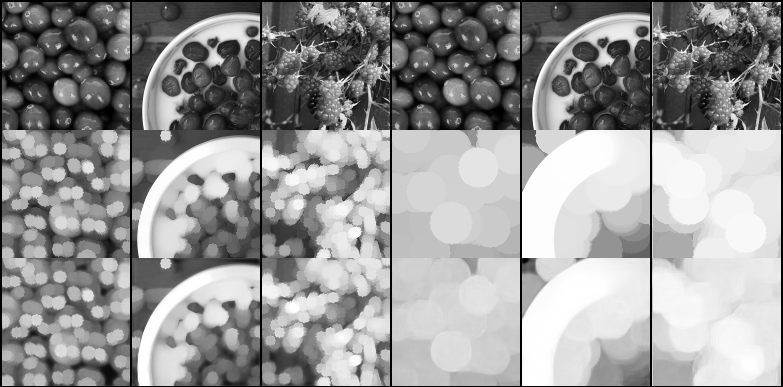
\includegraphics[width=0.85\linewidth]{fig/disk fixed.png}
\caption{Approximation of grayscale morphology with the disk structuring element and fixed parameters (1-st row: original images, 2-st row: morphological dilation, 3-st row: neural network). The first three images correspond to dilation with a radius of 5, while the second three correspond to dilation with a radius of 20. Two networks were trained to approximate the morphological dilation with different radii independently.}
\label{figure:Morphology}
\end{figure*}


\begin{figure}[h!]
\centering
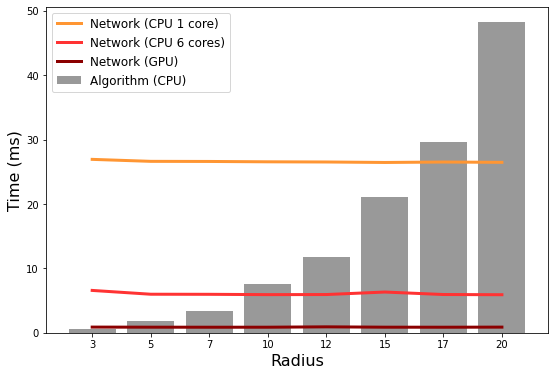
\includegraphics[width=1\linewidth]{fig/time.png}
\caption{Inference time of classical algorithm (disk-structured morphological dilation) and its neural approximation with (unparameterized) ResNet. The CPU algorithm implementation is single-threaded.}
\label{figure:InferenceTime}
\end{figure}


% \begin{figure*}[h]
% \centering
% 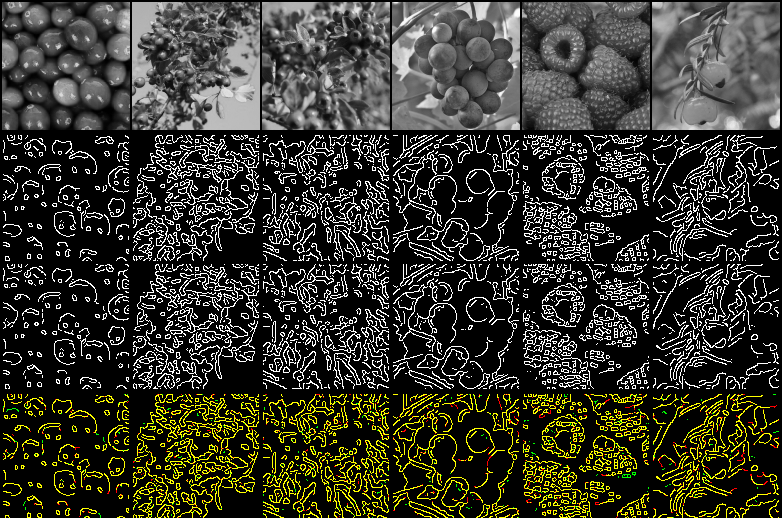
\includegraphics[width=0.8\linewidth]{fig/canny fixed.png}
% \caption{Approximation of Canny edge detector with fixed parameters (1-st row: original images, 2-st row: Canny edge detector, 3-st row: neural network, 4-st row: pixel difference)}
% \label{figure:Canny}
% \end{figure*}


% \begin{figure*}[h]
% \centering
% 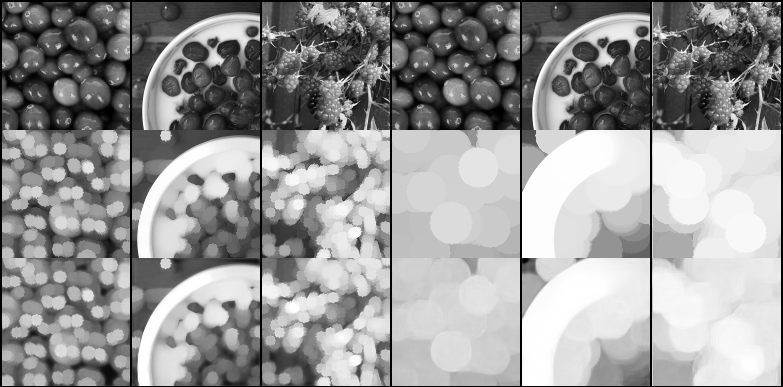
\includegraphics[width=0.8\linewidth]{fig/disk fixed.png}
% \caption{Approximation of grayscale morphology with the disk structuring element and fixed parameters (1-st row: original images, 2-st row: morphological dilation, 3-st row: neural network)}
% \label{figure:Morphology}
% \end{figure*}

\begin{figure*}[h]
\centering
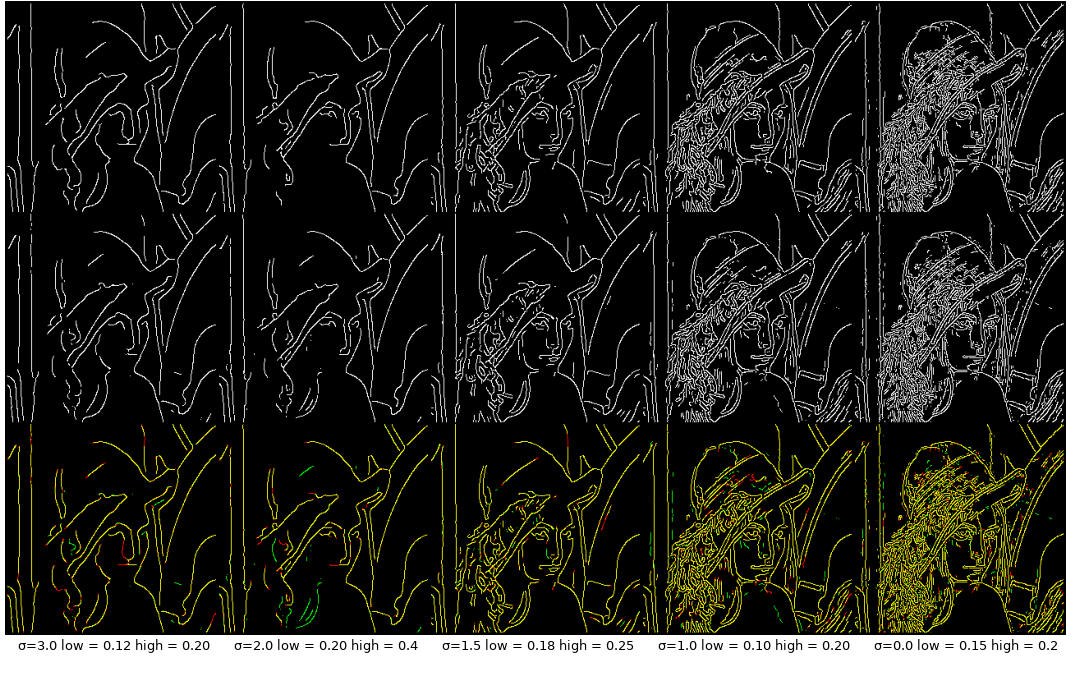
\includegraphics[width=0.85\linewidth]{fig/par-canny.png}
\caption{Parameterized approximation of Canny edge detector (1-st row: Canny edge detector, 2-st row: neural network, 3-st row: pixel difference, where black, yellow, green, and red colours stand for true negative, true positive, false positive, and false negative pixels, respectively).}
\label{figure:ParCanny}
\end{figure*}

\begin{figure*}[h]
\centering
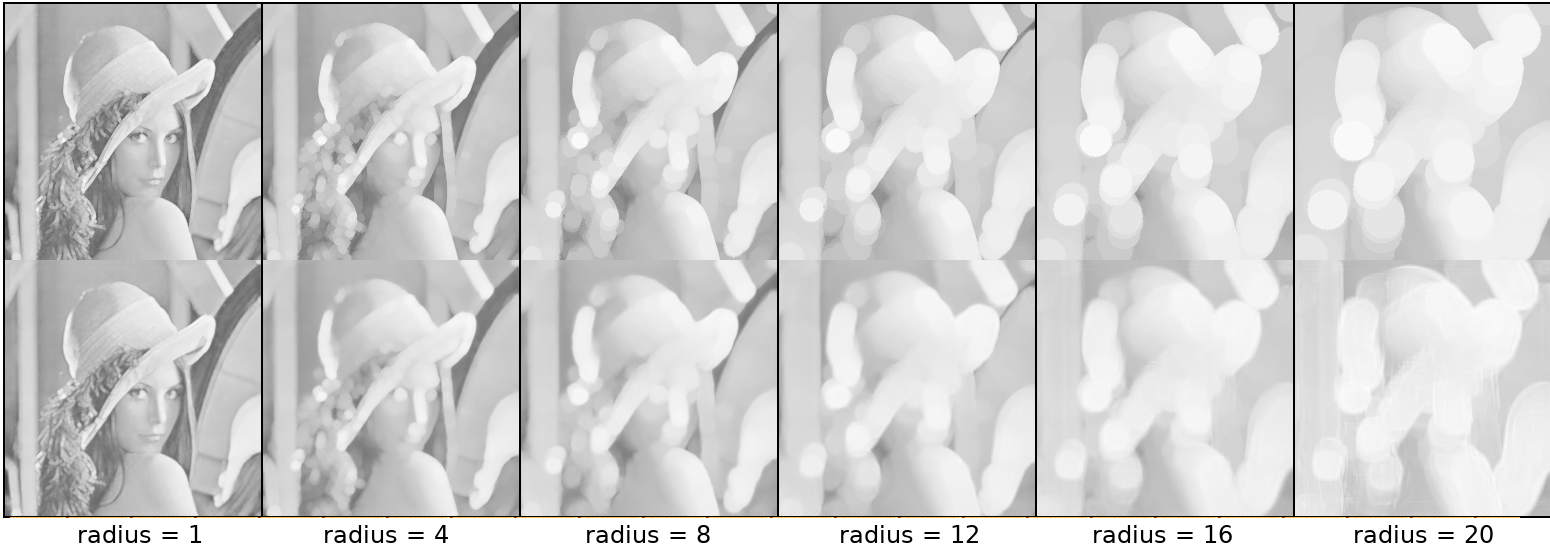
\includegraphics[width=0.85\linewidth]{fig/lena disk.png}
\caption{Parameterized approximation of grayscale morphology with the disk structuring element (1-st row: morphological dilation, 2-st row: neural network).}
\label{figure:ParMorphology}
\end{figure*}



Moreover, we compared inference times of the ResNet (fig.  \ref{figure:InferenceTime}) with the skimage.morphology (v.0.17.2) implementation and noticed that starting from a certain radius, neural network approximation works faster than the classical algorithm even in single-threaded inference mode.
In fully parallel GPU inference, the ResNet is faster than the CPU implementation in all cases, and while such performance comparison is unfair, it illustrates one of the benefits of NN approximations, which is the availability of highly parallelized implementations. 
It is worth mentioning that we did not apply any optimization techniques to speed up inference of the ResNet, while there is a more computational efficient implementation of it (e.g.  \cite{ResNetDetection}, which provides a threefold increase in the inference performance). The parameters of the testing system are: Intel(R) Xeon(R) W-2133 CPU @ 3.60GHz, 6 cores, 12 threads; GeForce RTX 2080 Ti 11 Gb GPU.
% \begin{itemize}
%     \item[--] Architecture: x86\_64;
%     \item[--] CPU op-mode(s):      32-bit, 64-bit;
%     % \item[--] Thread(s) per core:  2
%     % \item[--] Core(s) per socket:  6
%     % \item[--] Socket(s):           1
%     \item[--] CPU model name: Intel(R) Xeon(R) W-2133 CPU @ 3.60GHz;
%     \item[--] GPU model name: GeForce RTX 2080 Ti 11 Gb.
% \end{itemize}

Thus, we found that typical neural network architectures are able to approximate at least some of the typical image processing algorithms, while having few enough weights to be computationally competitive with purpose-built algorithms. 


\subsection*{\textbf{Parameterized approximation}}

An important property of classical image processing algorithms is parameterization, therefore they can be customized for a particular task while neural networks usually implement a fixed operation. In real-world applications, it is often necessary for a developer or a user to be able to tune the parameters. That is why another aim of our research is to consider the approaches to the parameterization of neural networks. We decided to start with the simplest approach, which is adding filter parameters as auxiliary channels of an input image.  

% Canny detector has three key parameters: sigma, low threshold, and high threshold. The high threshold was parameterized via the low threshold multiplied by a coefficient $k$. We consider these parameters as independent uniformly distributed random variables with a range:
% \begin{itemize}
%     \item[--] $\sigma$: $0 - 3$;
%     \item[--] low threshold: $0.1 - 0.2$;
%     \item[--] $k$: $1.05 - 2$.
% \end{itemize}

Canny detector has three key parameters: sigma, low threshold, and high threshold. The high threshold was parameterized via the low threshold multiplied by a coefficient $k$. We consider these parameters as independent uniformly distributed in the interval [0; 3] for sigma, [0.1; 0.2] for low threshold, and [1.05; 2] for $k$, random variables.

Since the distribution is multidimensional and its components are independent, it is crucial to sample from it with as maximum coverage of the probability space as possible. Latin hypercube sampling (LHS), proposed by \cite{LHS}, ensures that the set of samples is a very good representative of the real variability. That is why we used it for sampling the set of parameters during training phase. 

The training was organised as follows: at each epoch, we sampled 1000 sets of parameters with LHS. For each image from the training set, we randomly chose a set of parameters and added its values to the channels of the image. Since there are 6000 images in the training set, each set of parameters was applied to roughly six images. In the case of continuous random variables, the number of possible sets of parameters is infinite, that is why it makes sense to increase the number of epochs so that the network "see" as many sets of parameters as possible and learn how to approximate them. We trained our model for 200 epochs, which means there were 200000 sets of parameters. Also, we had to increase the number of convolutional kernels in the hidden layers from 12 to 16 compared to the unparameterized version. A visualization of the ResNet work is shown in the fig. \ref{figure:ParCanny}. A dependence on the parameters is pronounced, but the quality of the approximation is slightly reduced compared to the approximation with fixed parameters. The Matthew's correlation coefficient is 0.8917 and IoU is 0.9021. 

% \begin{figure*}[h!]
% \centering
% 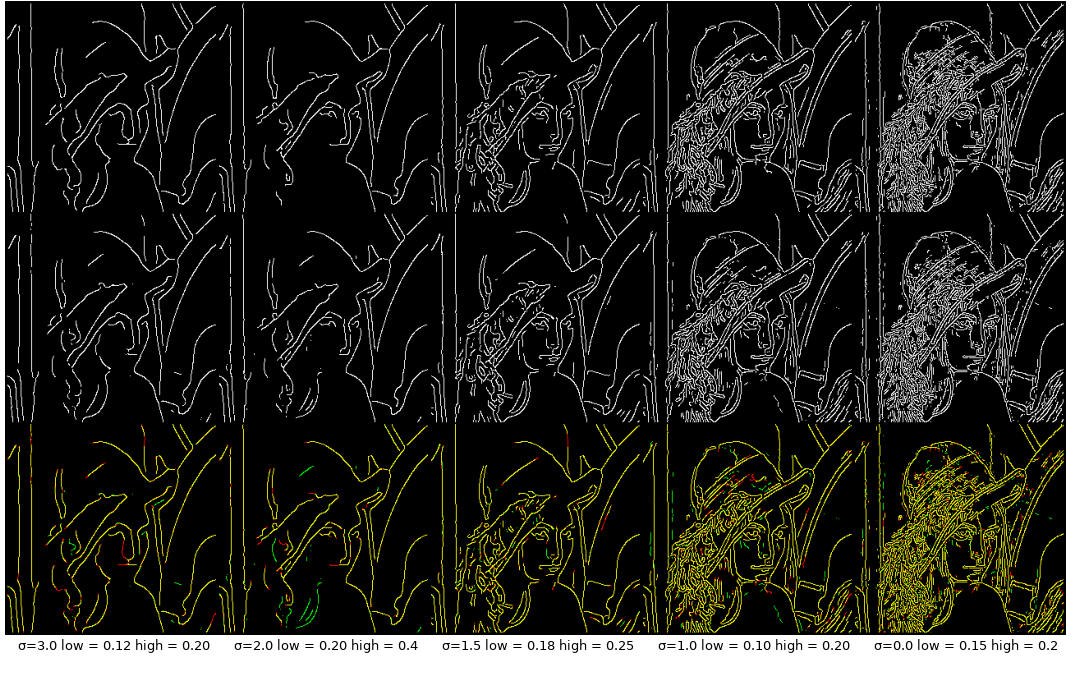
\includegraphics[width=1\linewidth]{fig/par-canny.png}
% \caption{Parameterized approximation of Canny edge detector}
% \label{figure:ParCanny}
% \end{figure*}

Disk-structured morphological dilation has one parameter, which is the radius of the disk. As long as the radius must be a positive integer, we consider it a discrete random variable, uniformly distributed in the interval [1; 20]. The model was trained in the same way as the Canny approximation network, but we did not use LHS because it is not necessary in case of one-dimensional discrete probability space. A visualization of the ResNet work is shown in the fig. \ref{figure:ParMorphology}. 

% \begin{figure*}[h!]
% \centering
% 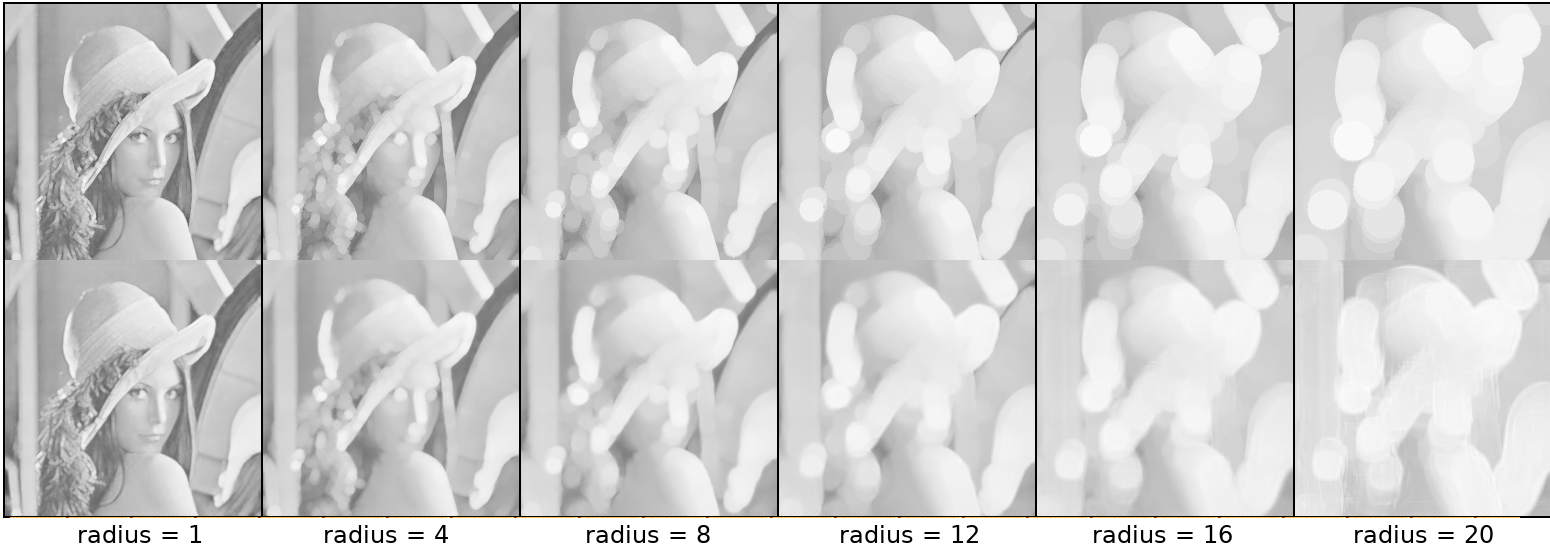
\includegraphics[width=1\linewidth]{fig/lena disk.png}
% \caption{Parameterized approximation of grayscale morphology with the disk structuring element}
% \label{figure:ParMorphology}
% \end{figure*}


Approximation of Canny edge detector and morphological dilation showed that the simplest parameterization approach via channels of input image works well enough for some applications.


